\documentclass{article}
\usepackage[lmargin=3cm, tmargin=3cm, rmargin=2cm, bmargin=2cm]{geometry}
\usepackage[onehalfspacing]{setspace}
\usepackage[utf8]{inputenc}
\usepackage[T1]{fontenc}
\usepackage[brazil]{babel}
\usepackage{amsmath, bbm}
\usepackage{graphicx, graphics, xcolor, comment, enumerate, multirow, multicol, indentfirst}
\usepackage{hyperref}
\usepackage{float}

\title{MAP2212 - EP3 Métodos de integração de Monte Carlo (Quase Aleatório}
\author{Vinícius da Costa Collaço - 11811012}
\date{Maio de 2022}

\begin{document}

\maketitle

\section{Introdução}


Esse relatório visa apresentar uma solução para o segundo exercício programa (EP3) proposto na matéria MAP2212/2022 (Laboratório de Computação e Simulação) do curso de bacharelado de matemática aplicada e computacional (BMAC) do instituito IME-USP.

O objetivo é implementar quatro variantes do método estocástico de integração de Monte Carlo, com um gerador de número quase aleatórios, para integrar a função $f(x) = \exp{(-ax)}\cos{(bx)}$ no intervalo $[0,1]$, onde $a = 0,RG, b = 0,CPF$. RG e CPF são os números de identificação do autor. Para proteção dos dados do autor, serão utilizados somente 6 dígitos significativos do RG e CPF, essa alteração não traz mudança significativa na função ou nos métodos utilizados.

Portanto, a integral cujo o valor será estimado será:

\begin{equation}
    \gamma = \int_0^1 e^{-0.460279x}\cos{(0,382023x)} dx
    \label{eqn:integral}
\end{equation}

A estimativa da integral deverá ser calculada com um erro mínimo de:

\begin{equation}
    \frac{|{\hat{\gamma}-\gamma}|}{\gamma} \leq 0.0005
    \label{eqn:erro}
\end{equation}

Utilizando a linguagem \textit{Python} e bibliotecas adequadas\cite{harris2020array, Waskom2021, Hunter:2007, 2020SciPy-NMeth, FEINBERG201546}, a integral em \ref{eqn:integral} será estimada utilizando os seguintes métodos de Monte Carlo:


\begin{enumerate}
    \item \textit{Crude}
    \item \textit{Hit or Miss}
    \item \textit{Importance Sampling}
    \item \textit{Control Variates}
\end{enumerate}

\section{Implementação do gerador de números quase aleatórios}

Para a geração de números quase aleatórios desse EP, será utilizada a biblioteca chaospy\cite{FEINBERG201546}, com a geração de uma sequência de baixa discrepância Sobol, tendo o algoritmo implementado na própria biblioteca.

No EP será necessária a execução de duas distribuições distintas; a distribuição uniforme e a distribuição exponencial truncada. Para comparação visual foi gerada na figura\ref{fig:Comp_pseudo_quase} pontos com as distribuições uniforme e exponencial truncada em [0,1] e com os geradores pseudo aleatório e quase aleatório.

\begin{figure}[H]
    \centering
    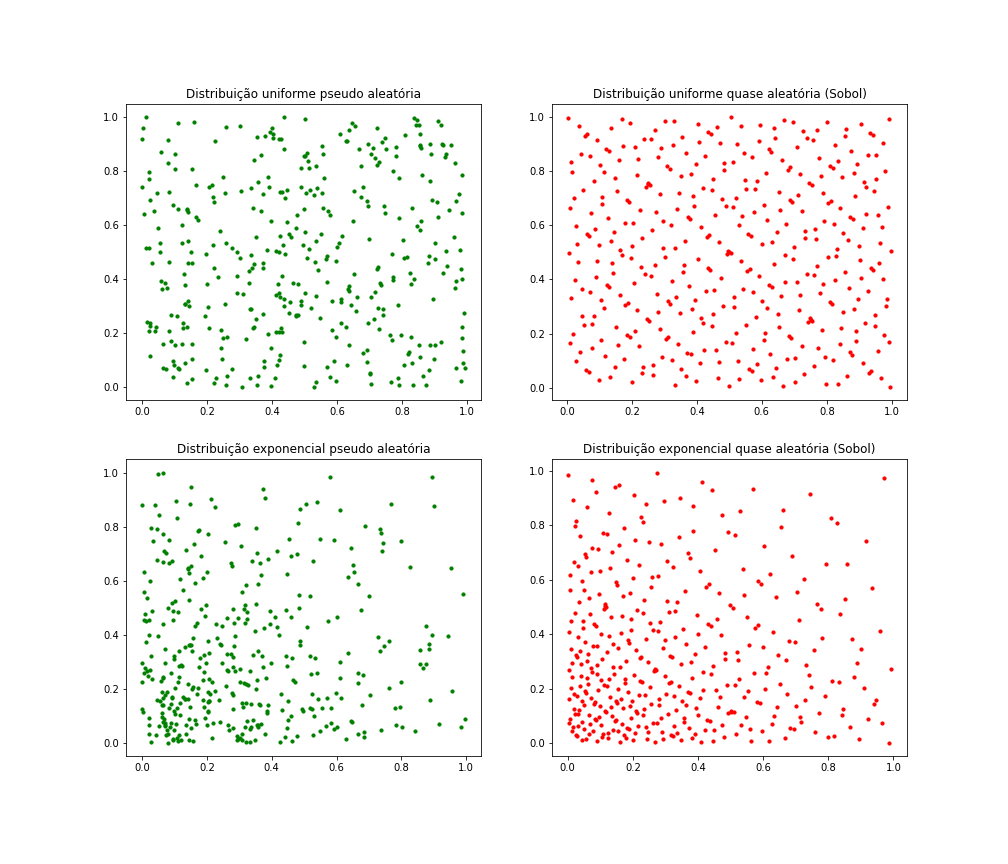
\includegraphics[width=.9\linewidth]{Imagens/Comparacao_Distribuicao.png}
    \caption{Comparação dos geradores pseudo aleatório e quase aleatório}
    \label{fig:Comp_pseudo_quase}
\end{figure}

Mesmo com distribuições distintas pôde-se observar pontos "mais bem comportados" com o gerador de números quase aleatórios.

\section{Definindo o tamanho da amostra (n)}

Para a definição do valor do n, iremos utilizar a aproximação assintótica de uma distribuição Bernoulli.

Supondo que o tamanho da amostra seja relativamente grande, pelo teorema do limite central, podemos aproximar a Bernoulli por uma normal, tendo:

\[
P(|\hat{p} - p|\leq \varepsilon)\geq \gamma 
\] \cite{estatbas}

\[
P(-\varepsilon \leq \hat{p} - p \leq \varepsilon) = P\left( \frac{-\sqrt{n}\varepsilon}{\sigma} \leq Z \leq \frac{\sqrt{n}\varepsilon}{\sigma}\right) \approx \gamma
\]
obtendo finalmente 

\begin{equation}
    n = \frac {\sigma^2 {Z_\gamma}^2} {\varepsilon^2}
    \label{eqn:valorn}
\end{equation}

esse resultado obtido em \ref{eqn:valorn} será utilizado nos quatro métodos

\subsection{Intervalo de confiança}
Para o problema será utilizado um intervalo de confiança $\gamma = 95\%$, escolhido arbitrariamente obtendo assim o $Z_\gamma$ da $N(0,1)$, portanto $Z_\gamma = 1,96$ e será utilizado nos quatro métodos.

\subsection{Erro amostral $(\varepsilon)$}

O erro amostral é dado por $|\hat{\gamma}-{\gamma}|$ com o erro exigido pelo problema em \ref{eqn:erro}, temos que o erro amostral será dado por:

\begin{equation*}
    \varepsilon = 0.0005\cdot\gamma
\end{equation*}

porém como não sabemos o valor real de gamma, será utilizado o estimador $\hat{\gamma}$ para cálculo do erro amostral, portanto o erro amostral será dado por:
\begin{equation}
    \varepsilon = 0.0005\cdot\hat{\gamma}
    \label{eqn:erroamostral}
\end{equation}

o valor do estimador será obtido em cada método através de uma amostra piloto. Para meios de comparação será utilizado o mesmo tamanho de amostra para o piloto, que será descrito nas próximas seções. 

\subsection{Variância}

Para obtenção da variância, em cada método será utilizada a variância amostral $(\hat{\sigma}^2)$ obtida a partir da amostra piloto

\subsection{Amostra Piloto}

Para o tamanho da amostra piloto foi escolhido arbitrariamente $n=100$

\section{Método \textit{Crude}}

\begin{figure}[H]
    \centering
    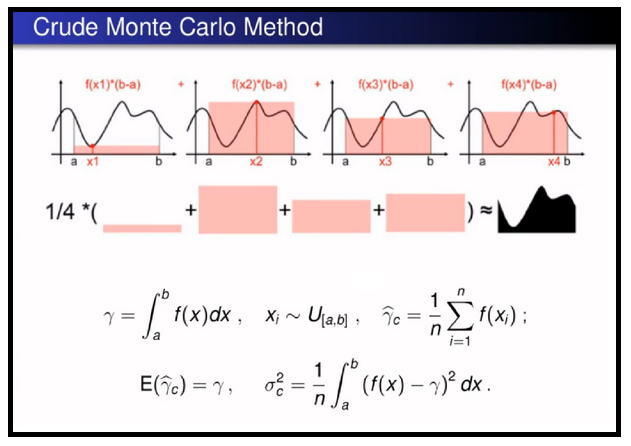
\includegraphics[width=.7\linewidth]{Imagens/MC_Crude.png}
    \caption{Método Crude}
    \label{fig:Crude}
\end{figure}

Um resumo do método \textit{Crude} pode ser observado na figura \ref{fig:Crude} 

\subsection{Estimador $\hat{\gamma_c}$ inicial}
Para o cálculo do $\hat{\gamma_c}$ será utilizado um método empírico, uma amostra piloto na função crude(Seed,n), com $n=100$ e $Seed=38$, para ser possível a replicação.
Resultando em $$\hat{\gamma_c} = 0.784909$$

\subsection{Variância amostral no Método \textit{Crude}}
Para o cálculo das variâncias empíricas foi criada a função variancias (Seed, n), retornando a variância de cada método. As variâncias poderiam ser retornadas nas funções principais, mas optou-se por criar outra função para que as funções que foram exigidas no exercício retornassem somente os valores como foram descritos.

Para o método \textit{Crude}, a variância pode ser calculada por:

\begin{equation*}
    \hat{\sigma_c}^2 = \frac{1}{n-1}\sum_{i=1}^n (f(x) - \hat{\gamma_c})^2
\end{equation*}

Com $Seed=38$ e $n=100$, a variância amostral calculada na função variancia, resultou em:

$$\hat{\sigma_c}^2 = 0,0141315$$

Com o resultado obtido em \ref{eqn:erro}, temos:

\subsection{Erro amostral \textit{Crude} ($\varepsilon_c$)}

\begin{equation*}
    \varepsilon_c = 0,0005\cdot\hat{\gamma} = 0,0005\cdot0,784909 = 0,000392455 
\end{equation*}

\subsection{Cálculo do n para o método \textit{Crude} $(n_c)$}

O cálculo do n pode ser obtido através da equação em \ref{eqn:valorn}, com os valores amostrais obtidos anteriormente, temos:

\begin{equation*}
    n_c = \frac{0,0141315\cdot1,96^2}{0,000392455^2} = 352468,75
\end{equation*}

portanto:

\[
    n_c = 352469
\]



\section{Método \textit{Hit or Miss}}

\begin{figure}[H]
    \centering
    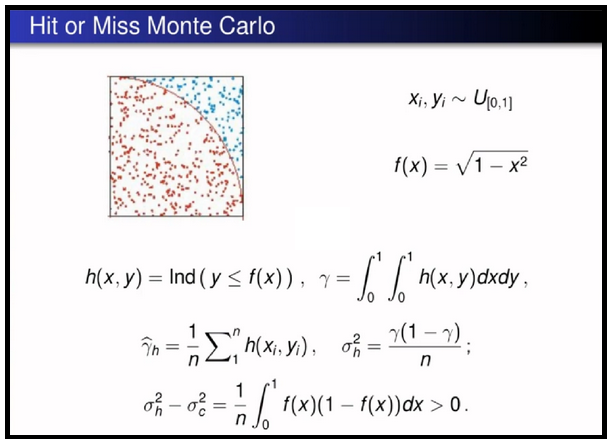
\includegraphics[width=.7\linewidth]{Imagens/MC_HoM.png}
    \caption{Método Hit or Miss}
    \label{fig:HoM}
\end{figure}

Um resumo do método \textit{Hit or Miss} pode ser observado na figura \ref{fig:HoM} 


\subsection{Estimador $\hat{\gamma}_{hom}$ inicial}
Para o cálculo do $\hat{\gamma}_{hom}$ será utilizado um método empírico, uma amostra piloto na função hit\_or\_miss(Seed,n), com $n=100$ e $Seed=38$, para ser possível a replicação, resultando em:
\[
    \hat{\gamma}_{hom} = 0,78
\]

\subsection{Variância amostral no Método \textit{Hit or Miss}}

Para o método \textit{Hit or Miss}, a variância pode ser calculada por:

\begin{equation*}
    \hat{\sigma}_{hom}^2 = \hat{\gamma}_{hom}(1-\hat{\gamma}_{hom})
\end{equation*}

Com $Seed=38$ e $n=100$, a variância amostral calculada na função variancia, resultou em:

\[
    \hat{\sigma}_{hom}^2 = 0,171599
\]
\subsection{Erro amostral \textit{Hit or Miss} ($\varepsilon_{hom}$)}

\begin{equation*}
    \varepsilon_{hom} = 0,0005\cdot\hat{\gamma} = 0,0005\cdot0,78 = 0,00039
\end{equation*}

\subsection{Cálculo do n para o método \textit{Hit or Miss} $(n_{hom})$}

O cálculo do n pode ser obtido através da equação em \ref{eqn:valorn}, com os valores amostrais obtidos anteriormente, temos:

\begin{equation*}
    n_{hom} = \frac{0,171599\cdot1,96^2}{0,00039^2} = 4334112,82
\end{equation*}

portanto:

\[
    n_{hom} = 4334113
\]


\section{Método \textit{Importance Sampling}}

\begin{figure}[H]
    \centering
    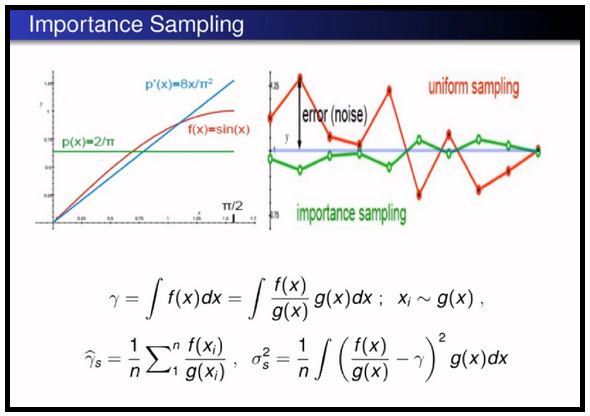
\includegraphics[width=.7\linewidth]{Imagens/MC_ImportanceSampling.png}
    \caption{Método Importance Sampling}
    \label{fig:ImpSam}
\end{figure}

Um resumo do método \textit{Importance Sampling} pode ser observado na figura \ref{fig:ImpSam}.\newline  

Para esse método utilizou-se a função de probabilidade exponencial truncada da biblioteca chaospy\cite{FEINBERG201546}, a função chaospy.TruncExponential, com parâmetros $upper = 1$ e $scale = 1/0.460279$, para resultar em uma $g(x)$, no intervalo $[0,1]$, da seguinte forma:

\begin{equation*}
    g(x) = \frac{0,460279\cdot \exp(-0,460279x)}{1-\exp(-0,460279)}
\end{equation*}

Dessa forma,

\begin{equation*}
    \frac{f(x)}{g(x)}=\frac{\exp(-0,460279x)\cdot\cos(0,382023x)}{\frac{0,460279\cdot \exp(-0,460279x)}{1-\exp(-0,460279)}}
\end{equation*}

Resultando em:

\begin{equation}
    \frac{f(x)}{g(x)} = \frac{\cos(0,382023x)\cdot(1-\exp(-0,460279))}{0,460279}
    \label{eqn:FsobreG}
\end{equation}


Essa a escolha da $g(x)$, simplificou algebricamente o resultado em \ref{eqn:FsobreG}, além de ser de fácil implementação da sua distribuição. Podemos observar a forte correlação no intervalo $[0,1]$ através da imagem \ref{fig:ImpSamDesmos}, gerada pela plataforma Desmos\cite{desmos}. 

\begin{figure}[H]
    \centering
    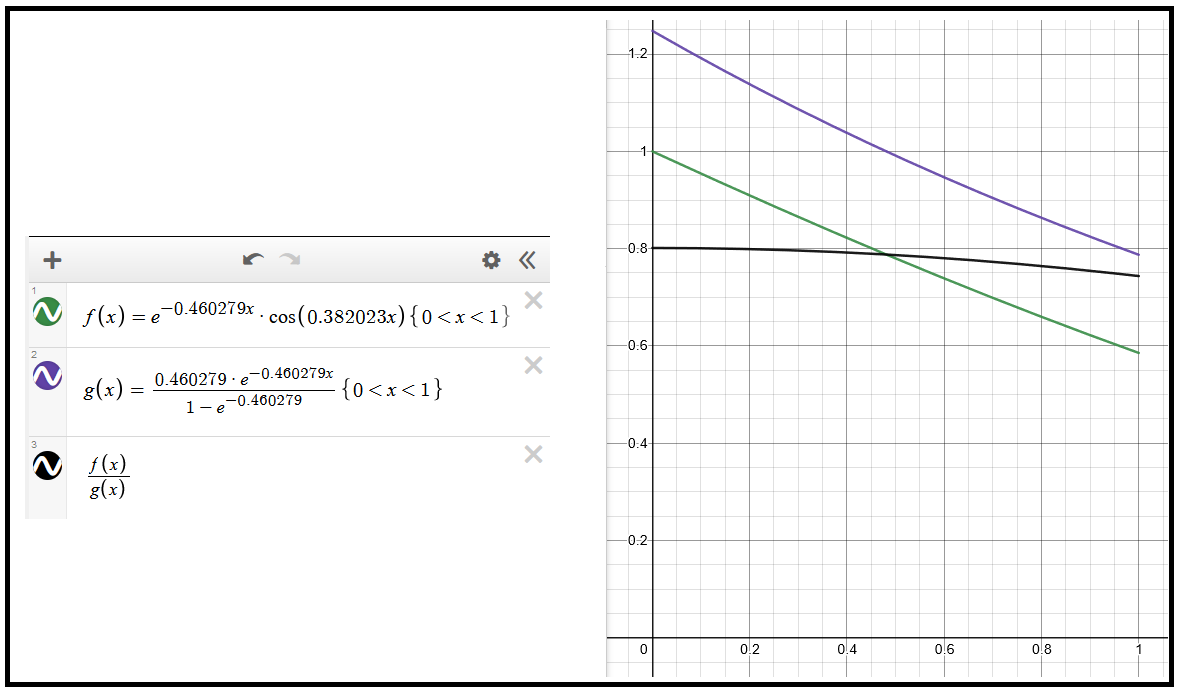
\includegraphics[width=.7\linewidth]{Imagens/Desmos_ImportanceSampling.png}
    \caption{Curvas do Importance Sampling gerada pela plataforma Desmos}
    \label{fig:ImpSamDesmos}
\end{figure}

Foi plotado também a equação \ref{eqn:FsobreG}, podendo ser observada um valor próximo da integral preterida.




\subsection{Estimador $\hat{\gamma}_{is}$ inicial}
Para o cálculo do $\hat{\gamma}_{is}$ será utilizado um método empírico, uma amostra piloto na função importance\_sampling(Seed,n), com $n=100$ e $Seed=38$, para ser possível a replicação, resultando em:
\[
    \hat{\gamma}_{is} = 0,784540
\]

\subsection{Variância amostral no Método \textit{Importance Sampling}}

Para o método \textit{Importance Sampling}, a variância foi calculada empiricamente com auxílio da função numpy.var() da biblioteca numpy \cite{harris2020array}, com grau de liberdade = 1:

Com $Seed=38$ e $n=100$, a variância amostral calculada na função variancia(), resultou em:

\[
    \hat{\sigma}_{is}^2 = 0,000271609
\]

\subsection{Erro amostral \textit{Importance Sampling} ($\varepsilon_{is}$)}

\begin{equation*}
    \varepsilon_{is} = 0,0005\cdot\hat{\gamma} = 0,0005\cdot0,784540 = 0,000392270
\end{equation*}

\subsection{Cálculo do n para o método \textit{Importance Sampling} $(n_{is})$}

O cálculo do n pode ser obtido através da equação em \ref{eqn:valorn}, com os valores amostrais obtidos anteriormente, temos:

\begin{equation*}
    n_{is} = \frac{0,000271609\cdot1,96^2}{0,000392270^2} = 6780,88
\end{equation*}

portanto:

\[
    n_{is} = 6781
\]



\section{Método \textit{Control Variates}}

\begin{figure}[H]
    \centering
    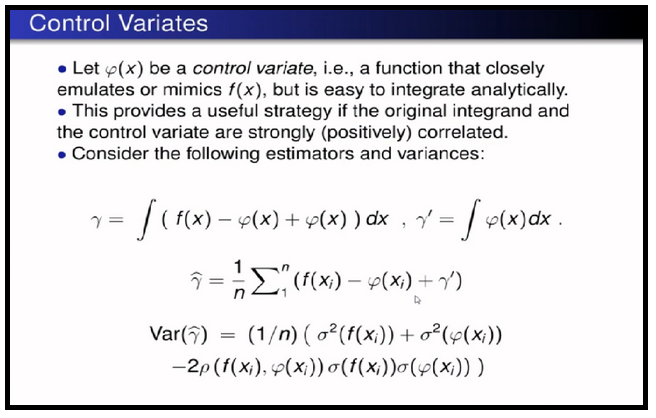
\includegraphics[width=.7\linewidth]{Imagens/MC_ControlVariates.png}
    \caption{Método Control Variates}
    \label{fig:ControlVar}
\end{figure}

Um resumo do método \textit{Control Variates} pode ser observado na figura \ref{fig:ControlVar}.
\newline
Para a escolha da função $\varphi(x)$ de controle, foi utilizado a ferramenta gráfica Desmos\cite{desmos}, para achar uma função com alta correlação e fácil integração no intervalo $[0,1]$.

\begin{figure}[H]
    \centering
    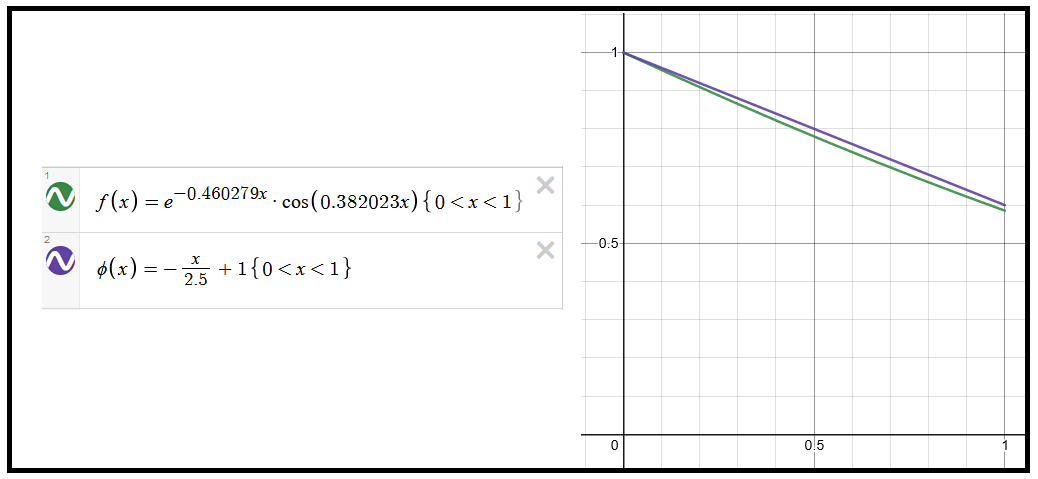
\includegraphics[width=.7\linewidth]{Imagens/Desmos_ControlVariate.png}
    \caption{Curvas da função $f(x)$ e $\varphi(x)$ pela plataforma Desmos}
    \label{fig:ControlVar_desmos}
\end{figure}

Optou-se por:

\begin{equation*}
    \varphi(x) = -\frac{x}{2,5}+1
\end{equation*}

Na figura \ref{fig:ControlVar_desmos} pode-se observar uma alta correlação entre as duas figuras.

\subsection{Integral de $\varphi(x)$}

\begin{equation*}
    \int_0^1{\varphi(x) dx} = \int_0^1{-\frac{x}{2,5}}dx+\int_0^1{1}dx = -0,2 + 1 = 0,8
\end{equation*}

\subsection{Estimador $\hat{\gamma}_{cv}$ inicial}
Para o cálculo do $\hat{\gamma}_{cv}$ será utilizado um método empírico, uma amostra piloto na função control\_variate(Seed,n), com $n=100$ e $Seed=38$, para ser possível a replicação, resultando em:
\[
    \hat{\gamma}_{cv} = 0,784190
\]

\subsection{Variância amostral no Método \textit{Control Variate}}

No método \textit{Control Variate} a variância pode ser calculada por:

\begin{equation*}
    var(\hat{\gamma}_{cv}) = (1/n) var(f(x))+var(\varphi(x) - 2\cdot cov(f(x), \varphi(x))
\end{equation*}

Como a variância de $f(x)$ e $\varphi(x)$ é desconhecida, foi calculada empiricamente a covariância amostral e as variâncias amostrais com auxílio da função numpy.var(), e numpy.cov() da biblioteca numpy \cite{harris2020array}, com grau de liberdade = 1:

Com $Seed=38$ e $n=100$, a variância amostral calculada na função variancia(), resultou em:

\[
    \hat{\sigma}_{cv}^2 = 0,0000336645
\]

\subsection{Erro amostral \textit{Control Variate} ($\varepsilon_{cv}$)}

\begin{equation*}
    \varepsilon_{cv} = 0,0005\cdot\hat{\gamma} = 0,0005\cdot0,784190 = 0,000392095
\end{equation*}

\subsection{Cálculo do n para o método \textit{Control Variate} $(n_{cv})$}

O cálculo do n pode ser obtido através da equação em \ref{eqn:valorn}, com os valores amostrais obtidos anteriormente, temos:

\begin{equation*}
    n_{cv} = \frac{0,0000352536\cdot1,96^2}{0,0003920953^2} = 841,20
\end{equation*}

portanto:

\[
    n_{cv} = 842
\]


\section{Resultados e discussões}

Para comparação dos métodos será utilizado o seguinte método de cálculo de eficiência: \cite{MCandQMCsampling}

\begin{equation*}
    Eff(\hat{\gamma}) = [MSE(\hat{\gamma}) \times C(\hat{\gamma})]^{-1} 
\end{equation*}

Como os estimadores são não-viesados a eficiência pode ser dada por:
\begin{equation*}
    Eff(\hat{\gamma}) = [{\hat{\sigma}}^2(\hat{\gamma}) \times C(\hat{\gamma})]^{-1}
\end{equation*}
onde ${\hat{\sigma}^2}(\hat{\gamma})$ é a variância do estimador e $C(\hat{\gamma})$ o tempo estimado para calcular $\hat{\gamma}$

Portanto quanto maior a eficiência melhor o método, contabilizando o tempo de execução, em consequência o algorítimo utilizado\newline


\begin{table}[H]
\begin{center}
    \begin{tabular}{|c|c|c|c|c|c|c|}
    \hline
                        & $\hat{\gamma}$ & Erro $\left( \frac{|\hat{\gamma}-\gamma|}{\gamma}\right)$ & $\hat{\sigma}^2(\hat{\gamma})$  & n       & $C(\hat{\gamma})$(s)    & Eficiência $(\hat{\gamma})$ \\ \hline
    Crude (pseudo)       & 0,784203 & $1,651\times10^{-4}$      & 0,01154    & 296596  & 0,02039   & 4246,2    \\ \hline
    Crude (sobol)       & 0,784280 & $1,547\times10^{-6}$      & 0,0141315    & 352469  & 1,7292   & 40,9    \\ \hline
    Hit or Miss (pseudo) & 0,784141 & $3,469\times10^{-4}$ & 0,1824     & 4852548 & 0,7539    & 7,3       \\ \hline
    Hit or Miss (sobol) & 0,784286 & $7,901\times10^{-6}$ & 0,171599     & 4334113 & 21,9554    & 0,26       \\ \hline
    Import. Samp. (pseudo) & 0,784316 & $6,765\times10^{-5}$ & 0,0002875  & 7187    & 0,0007908 & 4398001,2  \\ \hline
    Import. Samp. (sobol) & 0,784180 & $4,459\times10^{-8}$ & 0,000271609  & 6781    & 0,03504 & 105083,3  \\ \hline
    Control Variate (pseudo)   & 0,784143 & $7,975\times10^{-5}$ & 0,00003554 & 884     & 0,004347  & 6525271,3  \\ \hline
    Control Variate (sobol)    & 0,784274 & $7,767\times10^{-6}$ & 0,00003366 & 842     & 0,009617  & 3088758,1  \\ \hline
    \end{tabular}
    \caption{Tabela Comparativa}
    \label{tab:comparacao}
\end{center}
\end{table}

No geral tivemos uma redução de variância com o gerador de números pseudo aleatório sobol em comparação com o gerador pseudo aleatório e consequentemente uma redução da amostra para atingir o erro proposto, com exceção do método crude, isso pode ter ocorrido pela decisão inicial de se usar uma amostra inicial de apenas 100 amostras.

Como a integral proposta é de fácil cálculo, podemos obter o erro real, e no geral com o gerador quase aleatório tivemos erro menor, e bem pequeno. Tendo um indício que com uma amostra inicial maior o n poderia ter uma redução no geral.

Porém mesmo nos casos com menor variância e consequentemente n menor tivemos uma eficiência pior, pois o gerador de números quase aleatórios é mais lento que o gerador de números pseudo aleatórios.


\section{Conclusão}

A tarefa foi eficiente para mostrar o método de Monte Carlo nativo, e algumas variantes com redução de variância, além de aplicação de bibliotecas para geração de números pseudo aleatórios.
Na tabela \ref{tab:comparacao}, podemos observar que o método mais eficiente foi o método \textit{Control Variate}, seguido do \textit{Importance Sampling}, em ambos foi possível encontrar facilmente funções apropriadas e tal fato se mostrou efetivo nos resultados.
O método \textit{Crude} foi o método de mais fácil implementação, porém precisou de uma amostra grande para atingir o intervalo de confiança desejado. O método \textit{Hit or Miss} foi o com cálculo de variância mais fácil de se calcular, porém por ter um n grande e necessitar de dois arrays de pontos foi o método menos eficiente.


\newpage
\bibliographystyle{plain}
\bibliography{ref.bib}

\end{document}
